
\chapwithtoc{Introduction}

In today's era of information explosion and constant flow of information, it becomes more time-consuming to keep track of associations and understand the published content through media and online news, primarily when investing in a specific area. For instance, investing in a company like Apple acquiring and processing a wide range of available information requires significant effort and time investment in studying articles and other sources. 

Sentiment analysis, the ability to identify and evaluate the emotional charge of content, has evolved into a crucial instrument for comprehending opinions, attitudes, and the general atmosphere surrounding various topics. This work focuses on developing an application that allows users to visualize and analyze news sentiment using a knowledge graph network\textcolor{gray}{, even in real-time}.

Knowledge graphs are becoming an increasingly popular tool for representing and linking information. In our application, they are used to allow users not only to track the sentiment of individual reports but also to link and visualize relationships between companies through articles. In this way, users can gain a holistic view of world events and understand the interactions between entities.
This thesis will discuss the technical aspects of sentiment analysis and designing and implementing an application that conveys this information to users as efficiently as possible. \todo{Zeptat se - použití 1. osoby množného čísla nebo pasivní formy (it is required)} The aim is to provide users with a tool that allows them to actively monitor and analyze the flow of information about emotional overtones as one of the key identifiers in trading decisions. The thesis will be structured as follows. Chapter 1 will discuss the theoretical background behind the stock market. Chapter 2 will give an overview of data sources and the data itself. Chapter 3 will discuss the sentiment analysis and design of the application. Chapter 4 will discuss the implementation of the application. Chapter 5 will discuss the evaluation of the application. Chapter 6 will discuss the conclusion and future work.
\section*{Motivation}
\begin{figure}[htbp]
\centering
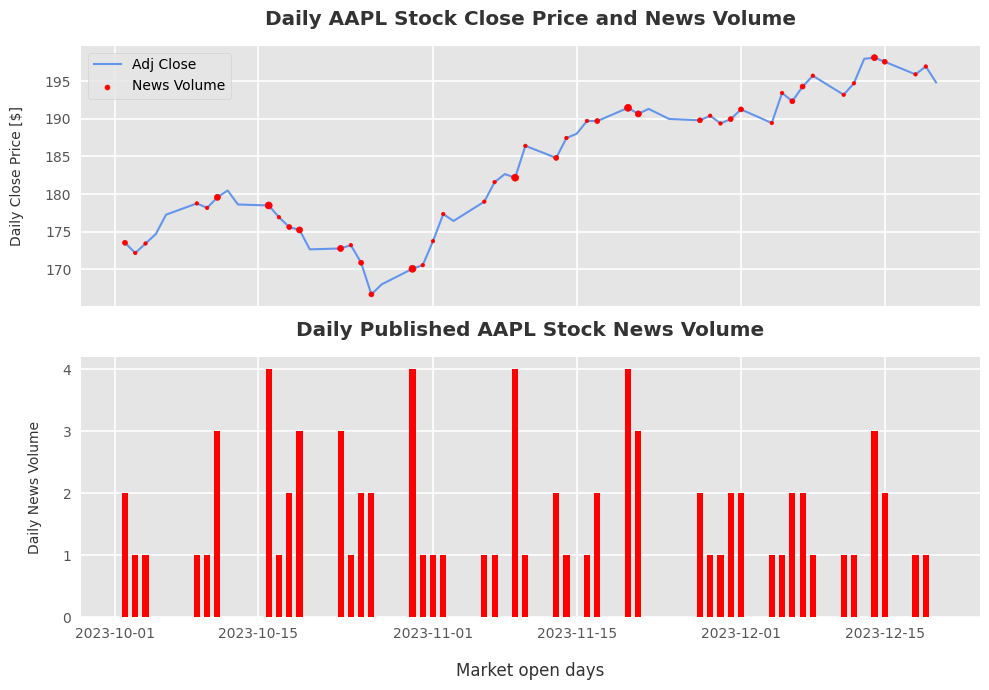
\includegraphics[width=1\linewidth]{img/motivation-sample.png}
\caption{This caption is a friendly reminder to never insert figures ``in text,'' without a floating environment, unless explicitly needed for maintaining the text flow (e.g., the figure is small and developing with the text, like some of the centered equations, as in). All figures \emph{must} be referenced by number from the text (so that the readers can find them when they read the text) and properly captioned (so that the readers can interpret the figure even if they look at it before reading the text --- reviewers love to do that).}
\label{fig:f}
\end{figure}

\section*{Related work}

\section*{How to write Introduction}
Introduction should answer the following questions, ideally in this order:
\begin{enumerate}
\item What is the nature of the problem the thesis is addressing?
\item What is the common approach for solving that problem now?
\item How this thesis approaches the problem?
\item What are the results? Did something improve?
\item What can the reader expect in the individual chapters of the thesis?
\end{enumerate}

Expected length of the introduction is between 1--4 pages. Longer introductions may require sub-sectioning with appropriate headings --- use \texttt{\textbackslash{}section*} to avoid numbering (with section names like `Motivation' and `Related work'), but try to avoid lengthy discussion of anything specific. Any ``real science'' (definitions, theorems, methods, data) should go into other chapters.
\todo{You may notice that this paragraph briefly shows different ``types'' of `quotes' in TeX, and the usage difference between a hyphen (-), en-dash (--) and em-dash (---).}

It is very advisable to skim through a book about scientific English writing before starting the thesis. I can recommend `\citetitle{glasman2010science}' by \citet{glasman2010science}.
